\section{Key elements of a kinect application}\label{4_1_requirements}
Microsoft created Kinect Human-Interface-Guidelines (HIG) for developer and designer that covers the design of basic and further interactions, gestures, voice, and feedback for an approriate kinect application~\cite{MicrosoftHIG2014-mh}. Therefore developer may follow this general standard to support their end-user. In the following key features of the guideline will be discussed on which the interactive slackline system will rely on to enhance the user experience.

\subsubsection{Context-awareness}
Controls should be placed where user would expect them to be. Also it is important that the user feel confident. Interactions should be designed simple and easy to learn.

\subsubsection{Visual and audio feedback}
Giving the user constant feedback helps people to know what is happening. Regarding this a combination of visual as well as audio feedback results in a better experience, e.g. clicking a button changes its visual state and provides an audio signal. More specific feedback regarding the system can be found in \textbf{\nameref{4_6_feedbackSystem}}.

\subsubsection{Clarification}
The user may interpret interactions with the system differently from others. Therefore the system should explain clearly what the user has to do, e.g. \textit{"Raise one hand above your head"} instead of just \textit{"Raise your hand"}. The cognitive load of the user should be kept low and not exceed a number of six gestures, such that she easily remembers the actions. The system has a set of three basic interaction techniques, which fits in this range.

\subsubsection{User viewer}
A small scene viewer shows the range in which the user can move and is recognized by the Kinect. It displays a mirror like view in which the user can see a silhouette of herself and the constraints of the Kinect device, like in figure \ref{fig:higUserViewer}.
\begin{figure}[htb]
	\centering
	\begin{minipage}[t]{1\linewidth}
		\centering
		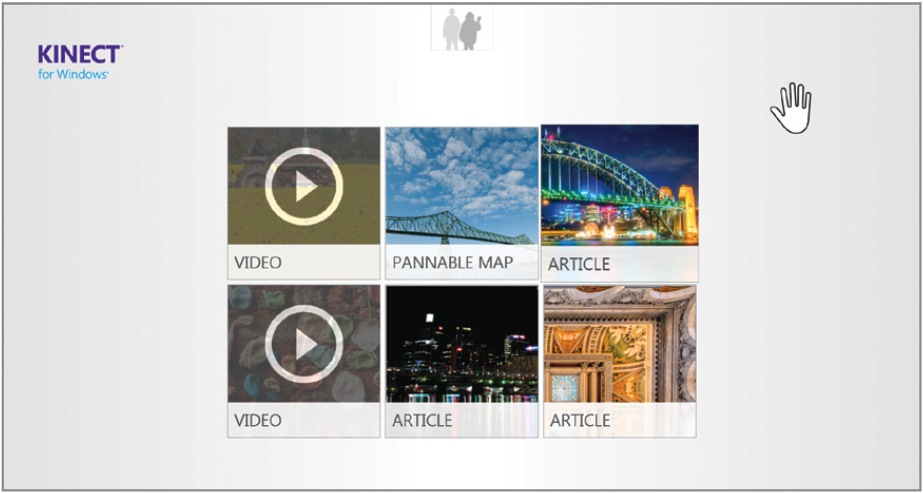
\includegraphics[width=0.79\linewidth]{Pictures/higUserViewer}
		\caption{User Viewer on top~\cite{MicrosoftHIG2014-mh}}
		\label{fig:higUserViewer}
	\end{minipage}
\end{figure}

\subsubsection{Learning interaction methods}
The system teach the user how to proper interact with it right from the beginning with an introduction tutorial. It provides also support to interact with both hands for left- and right-handed people. More about interaction methods can be seen in \textbf{\nameref{4_3_interaction}}.

\subsubsection{Teaching complex gestures / exercises}
For more complex gestures (exercises) the system provides a tutorial on how to accomplish this gesture successfully. An indicator should thereby show if the gesture is executed. More can be found in \textbf{\nameref{4_5_exercises}}.

\subsubsection{Element sizing}
The system will rely on the guidelines and match the button sizing regarding the screen resolution to keep reliability on interaction. This is a size of 208 by 208px in a resolution of 1920x1080 pixel. As recommended a tile button style will be used which are a good baseline where the user can hit them accurately and read the button text.

\subsubsection{Physical interaction zone}
This zone ensures that the user is able to reach anything in a comfortable range. In the application it is constrained by the joints of the shoulders to the hips of the opposite site of the interaction hand. It is designed like seen in figure \ref{fig:higPHIZ} to have a better understanding.
\begin{figure}[htb]
	\centering
	\begin{minipage}[t]{1\linewidth}
		\centering
		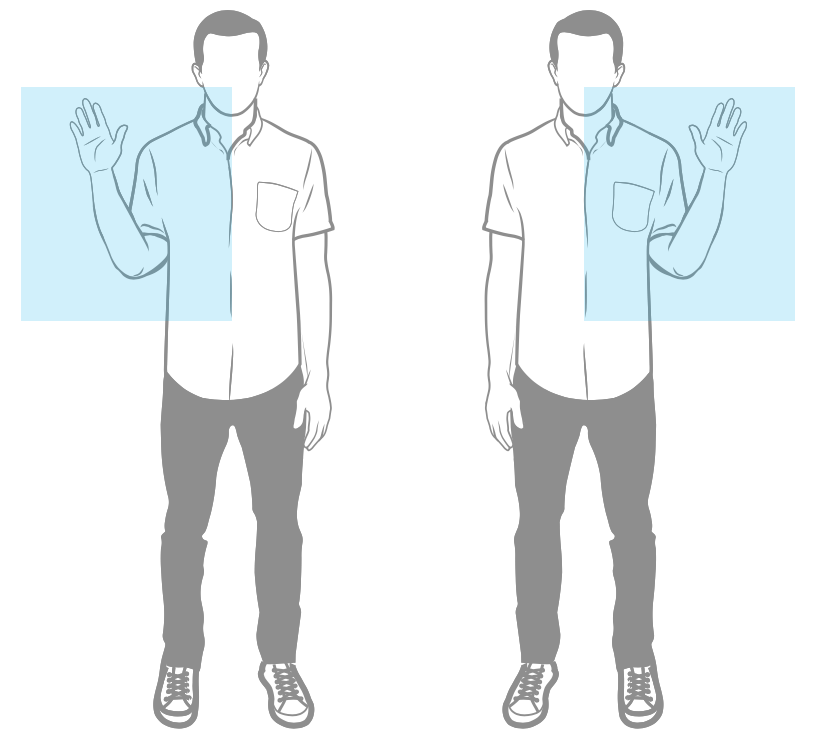
\includegraphics[width=0.5\linewidth]{Pictures/higPHIZ}
		\caption{Physical interaction zone~\cite{MicrosoftHIG2014-mh}}
		\label{fig:higPHIZ}
	\end{minipage}
\end{figure}

\begin{comment}
- System should provide a user view, such that the user knows the constraints of the kinect tracking area --> should be small if interacting in menu and big if needed in execution for example
\\- Audio feedback (success/failing)
\\- Big buttons/selectable elements
\\- Button state changes --> visualize
\\- \todo{picture of key elements from Kinect HIG}

- \todo{maybe combine interaction with key elements of a kinect application}
\end{comment}

\section{General}\label{4_2_general}
Since the user should get feedback about her performance during exercise execution, the system must be able to track her in an appropriate manner. Further all relevant data should be immediately saved when it is needed, for example when successfully accomplishing an exercise and so on. %unlocking exercise/stage, failing/accomplish exercise
In each screen there should be a title, which informs the user were she currently is. Also a back button gives her the possibility to go to the last screen if she misclicks. One can system that the system is available on one device but several persons should be able to interact with the system. Therefore it should provide a user selection screen, in which each user can select her own profile. This can also be seen in many others applications like \todo{[CITE]}
\begin{comment}
\\- system should be able to track user appropriately
\\- All relevant data should be immediately saved when it is needed (unlocking exercise/stage, failing/accomplish exercise)
\\- user should be able to go immediately to previous scene for almost all scenes --> back button
\\- Information about where the user currently is should be given --> title
\\\\- User selection
\end{comment}

\section{Interaction}\label{4_3_interaction}
Since the user can and should be able to navigate through the system by herself the interaction can be seen as one of the bigger parts of the system. The user can control a cursor with her own hand, which is also visualized in the screen. When initially starting the system the user should raise one hand over the head to convey that the system initially recognises and responds to a user action. 

Further a small tutorial is given in which the user is instructed in how to click by pushing his hand towards the Kinect or doing a point gesture and how to scroll through a menu. These actions have to be directly applied by the user. The state of the current interaction is visualized properly by providing a circle around the hand cursor that represents the progress like seen in figure \todo{insert figure}. Besides this she is instructed on how to stay in the right starting position. This is required by some actions like just before starting the exercise execution to ensure the user is ready.

Another big role of this plays in the exercise execution. Here the user interacts with the system to match a predefined gesture for accomplishing the exercise. Therefore real time feedback is provided which gives her hints about the right interaction and how good it is performed. More information about the feedback methods can be found in \textbf{\nameref{4_6_feedbackSystem}}.

\begin{comment}
- user can and should interact with the system
\\- Cursor visualization as hand image
\\- Engagement gesture for first interaction with Kinect (One hand over shoulder)
\\- She should be instructed how to interact 
\\- Different interaction methods should be provided to prevent failing on one (tutorial --> clicking (variations) + scrolling)
\end{comment}

\section{Stages}\label{4_4_stages}
The system contains predefined gestures, which are subdivided in stages, which can be seen in \textbf{\nameref{3_2_2_StagesExercises}}. A stage menu should be provided to give the user an overview and in which each one consists of several exercises. Every stage is locked except the first one, which is the users starting point. The next stage can be unlocked, by successfully executing all exercise in the current one. Hence it can be assured that the user is able to encounter with the more difficult exercises. The user should be introduced to the stage. In here the purpose, goal, and helpful techniques should be given, such that the user becomes an overview about the exercises. At last a summary scene shows several performance parameter for the exercises in this stage.
\begin{comment}
\\- system should provide predefined exercises that can be tracked per user
\\- A stage menu should be provided to the user, which shows her the amount of stages to complete
\\- It consists of 4 stages each with specific exercises (Preliminary, First contact with slacklining,  Static exercises, Dynamic exercises) like explained in chapter 3
\\- A stage consists of several exercises like explained in prev. chapter
\\- locked stages (initial first stage interactable)
\\- unlock stages (by successfully accomplishing all exercises from current stage)
\\- Stage introduction gives general information, describes the goal and tips for the current stage
-- a stage information scene provides her with the general introduction of this stage --> unlocks first exercise
\\- Stage summary contains average data about each exercise
\end{comment}

\section{Exercises}\label{4_5_exercises}
Each exercise is part of one stage. An exercise itself is divided into two body sides, which are further divided into several repetitions, see figure \ref{fig:exerciseStructure}. Each exercise is locked except the first one to provide a starting point. The next exercise can be unlocked by accomplishing both sides of the current exercise. Similarly a side is completed if all repetitions have been finished. Like for the stage, each exercise should be instructed for the user, such that she can successfully perform it. She should stand in a starting position to start the exercise. This is to ensure that no exercise is starting to track if the user would make a random gesture which could lead to confusion of the user. During the execution she should get real time feedback about her current performance, which is further discussed in \textbf{\nameref{4_6_feedbackSystem}}. After the execution a summary should show the performance of the execution with several parameters like execution time, amount of attempts needed, and the confidence regarding the given gesture.

\begin{figure}[htb]
	\centering
	\begin{minipage}[t]{1\linewidth}
		\centering
		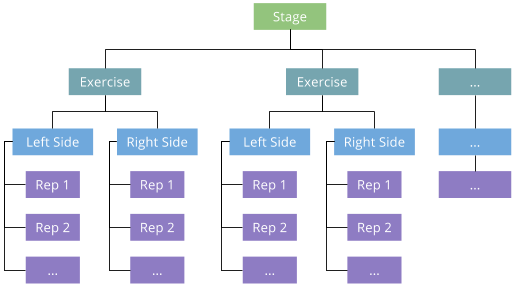
\includegraphics[width=1\linewidth]{Pictures/exerciseStructureTopDown2}
		\caption{Exercise structure~\cite{MicrosoftHIG2014-mh}}
		\label{fig:exerciseStructure}
	\end{minipage}
\end{figure}
\begin{comment}
\\\textbf{Exercises}
\\- System should provide predefined exercises that user can execute and her performance is tracked
\\- main menu / exercise selection
\\- lock / unlock 
\\- Each next exercise is unlocked if current exercise is successfully completed
\\- Each exercise counts as accomplished if both sides has been successfully trained
\\- click on exercise -> side selection - Each exercise consists of 2 sides, for train left and right side
\\- per exercise there should be an introduction on how to perform it successfully (instruction tip list, amount of repetitions, minimum time to hold a gesture, looping video)
\\- user has to stay in a starting position (both legs parallel to each other)
\\- exercise execution (user mirror)
\end{comment}

\section{Feedback system}\label{4_6_feedbackSystem}
Feedback is the main and most powerful component of the interactive learning system. Since the user should interact on her own with the system one has to assume that no other person interfere with her and the system. With this in mind the feedback of the system should designed in a way, that the user knows at anytime what she has to do or has done. In general audio and visual feedback is provided to the user. Regarding the \textbf{\nameref{4_3_interaction}} with the system, e.g. clicking a button, the system should respond with an audio signal and change the elements visual state accordingly.

For the accomplishment of exercise execution the system provides essential responses of the system like seen in other applications \todo {[cite, maybe Related Work]}. In the slackline system the following feedback indicators are integrated for the exercise execution:
\begin{itemize}
\item Staying in the right position before starting an exercise
\item When an exercise is currently correctly performed
\item How good the exercise is currently performed, namely the confidence
\item The elapsed time the user is performing the exercise
\item When the repetition is successfully accomplished, i.e. the minimum time has been reached
\item When an repetition attempt was not successful
\item How many repetitions in general, finished and left
\item Checklist about key elements in an execution (like hands up, foot stretched, etc.)
\item A summary that shows the user parameters about the performance (execution time, overall attempts, confidence) for each repetition and an average value of these
\item A similar summary can also be found for the entire stage, where the same parameters for each exercise are listed in average
\end{itemize}
With this a baseline is built for appropriate real time feedback to the user.

\begin{comment}
- in general audio and visual feedback
- if the user has clicked a button
- stays in the right position
- Indicator about if exercise is correctly executed
- Indicator about how good the exercise is performed
- real time feedback (Time, confidence, checklist, repetitions)
- system should inform how many repetitions are left
- system should inform when the repetition is successfully accomplished (audio, visual -> timer green, repetition counter)
- system should inform the user if repetition was not successful (audio, visual -> reset timer, checklist)
- After successful execution, a summary is shown about the performance of the user for each rep (time, attempts, confidence)
- tier summary (avg. time, attempts, confidence)
\end{comment}

\section{Scenario}\label{4_7_requirements_scenario}
To have a better understanding regarding the interplay of the several components a generic scenario workflow will be given from the point of view of the user:

The user raises the hands over her head to start the application. She is now instructed on how to interact with elements on  the screen, e.g. clicking and scrolling. After being confident with this, she selects her user profile to load the appropriate exercises and leads her to the stage selection. She selects the first stage since all others are currently locked. Now she is in the exercise menu. In here she clicks on the \textit{stage information} button, which gives her an introduction into the stage. After confirming that she has read the introduction the first exercise becomes unlocked and she selects it. After that she decides to train her left leg first in the side selection. An exercise introduction screen is following, which shows specific information about the execution. After reading the introduction she feels ready to counter the exercise. Therefore she goes into the starting position and starts the exercise by clicking the start button. The screen changes and all relevant elements are shown for the exercise execution. She performs every repetition of the exercise successfully. After finishing these the system leads her to the exercise summary screen, which shows her the performance of the just executed exercise. In here she can now decide to return to the main menu or go on and start the training for the other body side.

\begin{comment}
\todo{-maybe just user view scenario}
To have a better understanding regarding the interplay of the several components a generic scenario workflow will be given.
The user starts with an engagement gesture like raising her hand over the head to convey that the system initially recognises and responds to a user action. After that a tutorial about the interaction with the system will be given that covers clicking and scrolling techniques. Now she's confident with the system interaction and can select a profile in the user select to train. This loads the profile which leads to the stage selection menu. In here she can select a stage, whereas initially the first one is can be selected and the others have to be unlocked by successfully accomplishing all exercises in the preview stage. Selecting a stage leads to the exercise menu. In here she has to read initially the stage introduction to become a basic understanding about the exercises in here. After reading this, it unlocks the first exercise. Selecting an exercise leads to the side selection, where the user has to choose the side she wants to train for this exercise. This is followed by an introduction of the exercise, in which is explained how to perform it correctly. If the user is ready, she should stay in a starting position to be able to start the exercise execution. In here she find all relevant elements to perform the exercise, like indicators for the time, repetitions, confidence and a checklist, which helps her to correctly execute the exercise. After successfully executing the exercise, a summary is shown which summarizes the user performance. Then she can return to the main menu or directly approach the next exercise. A stage summary gives an overview about all exercises with average performance parameters.
\end{comment}

This procedure is also visualized in Figure \ref{fig:scenarioWorkflow} below.
\begin{figure}[htb]
	\centering
	\begin{minipage}[t]{1\linewidth}
		\centering
		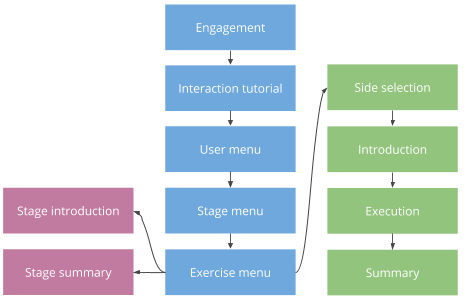
\includegraphics[width=0.79\linewidth]{Pictures/conceptScenarioFlow}
		\caption{Scenario workflow}
		\label{fig:scenarioWorkflow}
	\end{minipage}
\end{figure}